\documentclass[../main.tex]{subfiles}

\begin{document}
EU citizens engage in a wide range of activities online which include getting news, banking, social media, shopping and many more. According to the Digital Economy and Society Index (DESI), in 2019 Sweden, Denmark and the UK have the most advanced digital economies. On the other hand, Romania, Poland and Greece score the lowest in DESI \cite{desi_2019}.

Even though 85\% of Europeans used the internet in 2019, the COVID-19 pandemic is expected to contribute to the rise of the number of internet users as well as interactions and services \cite{desi_2020}. With the increase in internet usage, there has been a rise in the amount of information collected by websites, such as location data \cite{hern_2018}, as well as online tracking with the use of Third-Party Cookies (TPs) \cite{roesner_2012}. 

Thus, the rapid growth of the internet and its online services has brought a new set of challenges and risks to citizens and governments alike. While the EU and the UK have introduced legislation in an attempt to mitigate and control those risks, the privacy of internet users at risk on a daily basis. 

\section{Legislation}
The EU and the UK have implemented laws in an attempt to protect their citizens from mass-scale data collection. Furthermore, such legislation gives the ability to governments to bring companies to justice for mishandling personal information, as seen from the Cambridge Analytica scandal \cite{guardian_analytica}.

\subsubsection{European Union}
The General Data Protection Regulation (GDPR) is a data protection and privacy law in the European Union that came into effect in May 2018. The primary goal of the GDPR is to give the ability to citizens to control their personal information online. For instance, it allows users to request their data held by companies and also their data erased. Furthermore, websites are required to disclose if they have implemented data collection mechanisms, as well as how long the data is going to be retained for and whether they are going to be shared with third parties or outside the EU \cite{gdpr_legal_text}.

\subsubsection{United Kingdom}
The Data Protection Act of 2018, is a UK parliament Act that aims to update the data privacy laws in the United Kingdom \cite{dpa_2018} (Data Protection Act 2018). Furthermore, It has been written to complement the GDPR but it is not limited by the GDPR’s provisions. 

\section{Cookie Banners}
Cookie banners are pop-ups that appear when users visit a website. They can either take the full screen, forcing users to interact with them before continuing to the content or appear as small bars allowing users to bypass them. Figure \ref{fig:intro_cookie_guardian}, depicts the \say{full-screen} cookie banner of The Guardian (\url{https://theguardian.com}) and Figure \ref{fig:intro_cookie_york} shows the cookie notice implementation of the University of York’s (\url{https://york.ac.uk}) which does not force the user to interact with it. 

\begin{figure}[ht!]
    \centering
    \begin{subfigure}[b]{0.45\textwidth}
        
\includegraphics[width=\textwidth]{images/intro/guardian}
        \caption{The \say{full screen} cookie banner shown to The Guardian's visitors.}
        \label{fig:intro_cookie_guardian}
    \end{subfigure}
    \hfill
    \begin{subfigure}[b]{0.45\textwidth}
        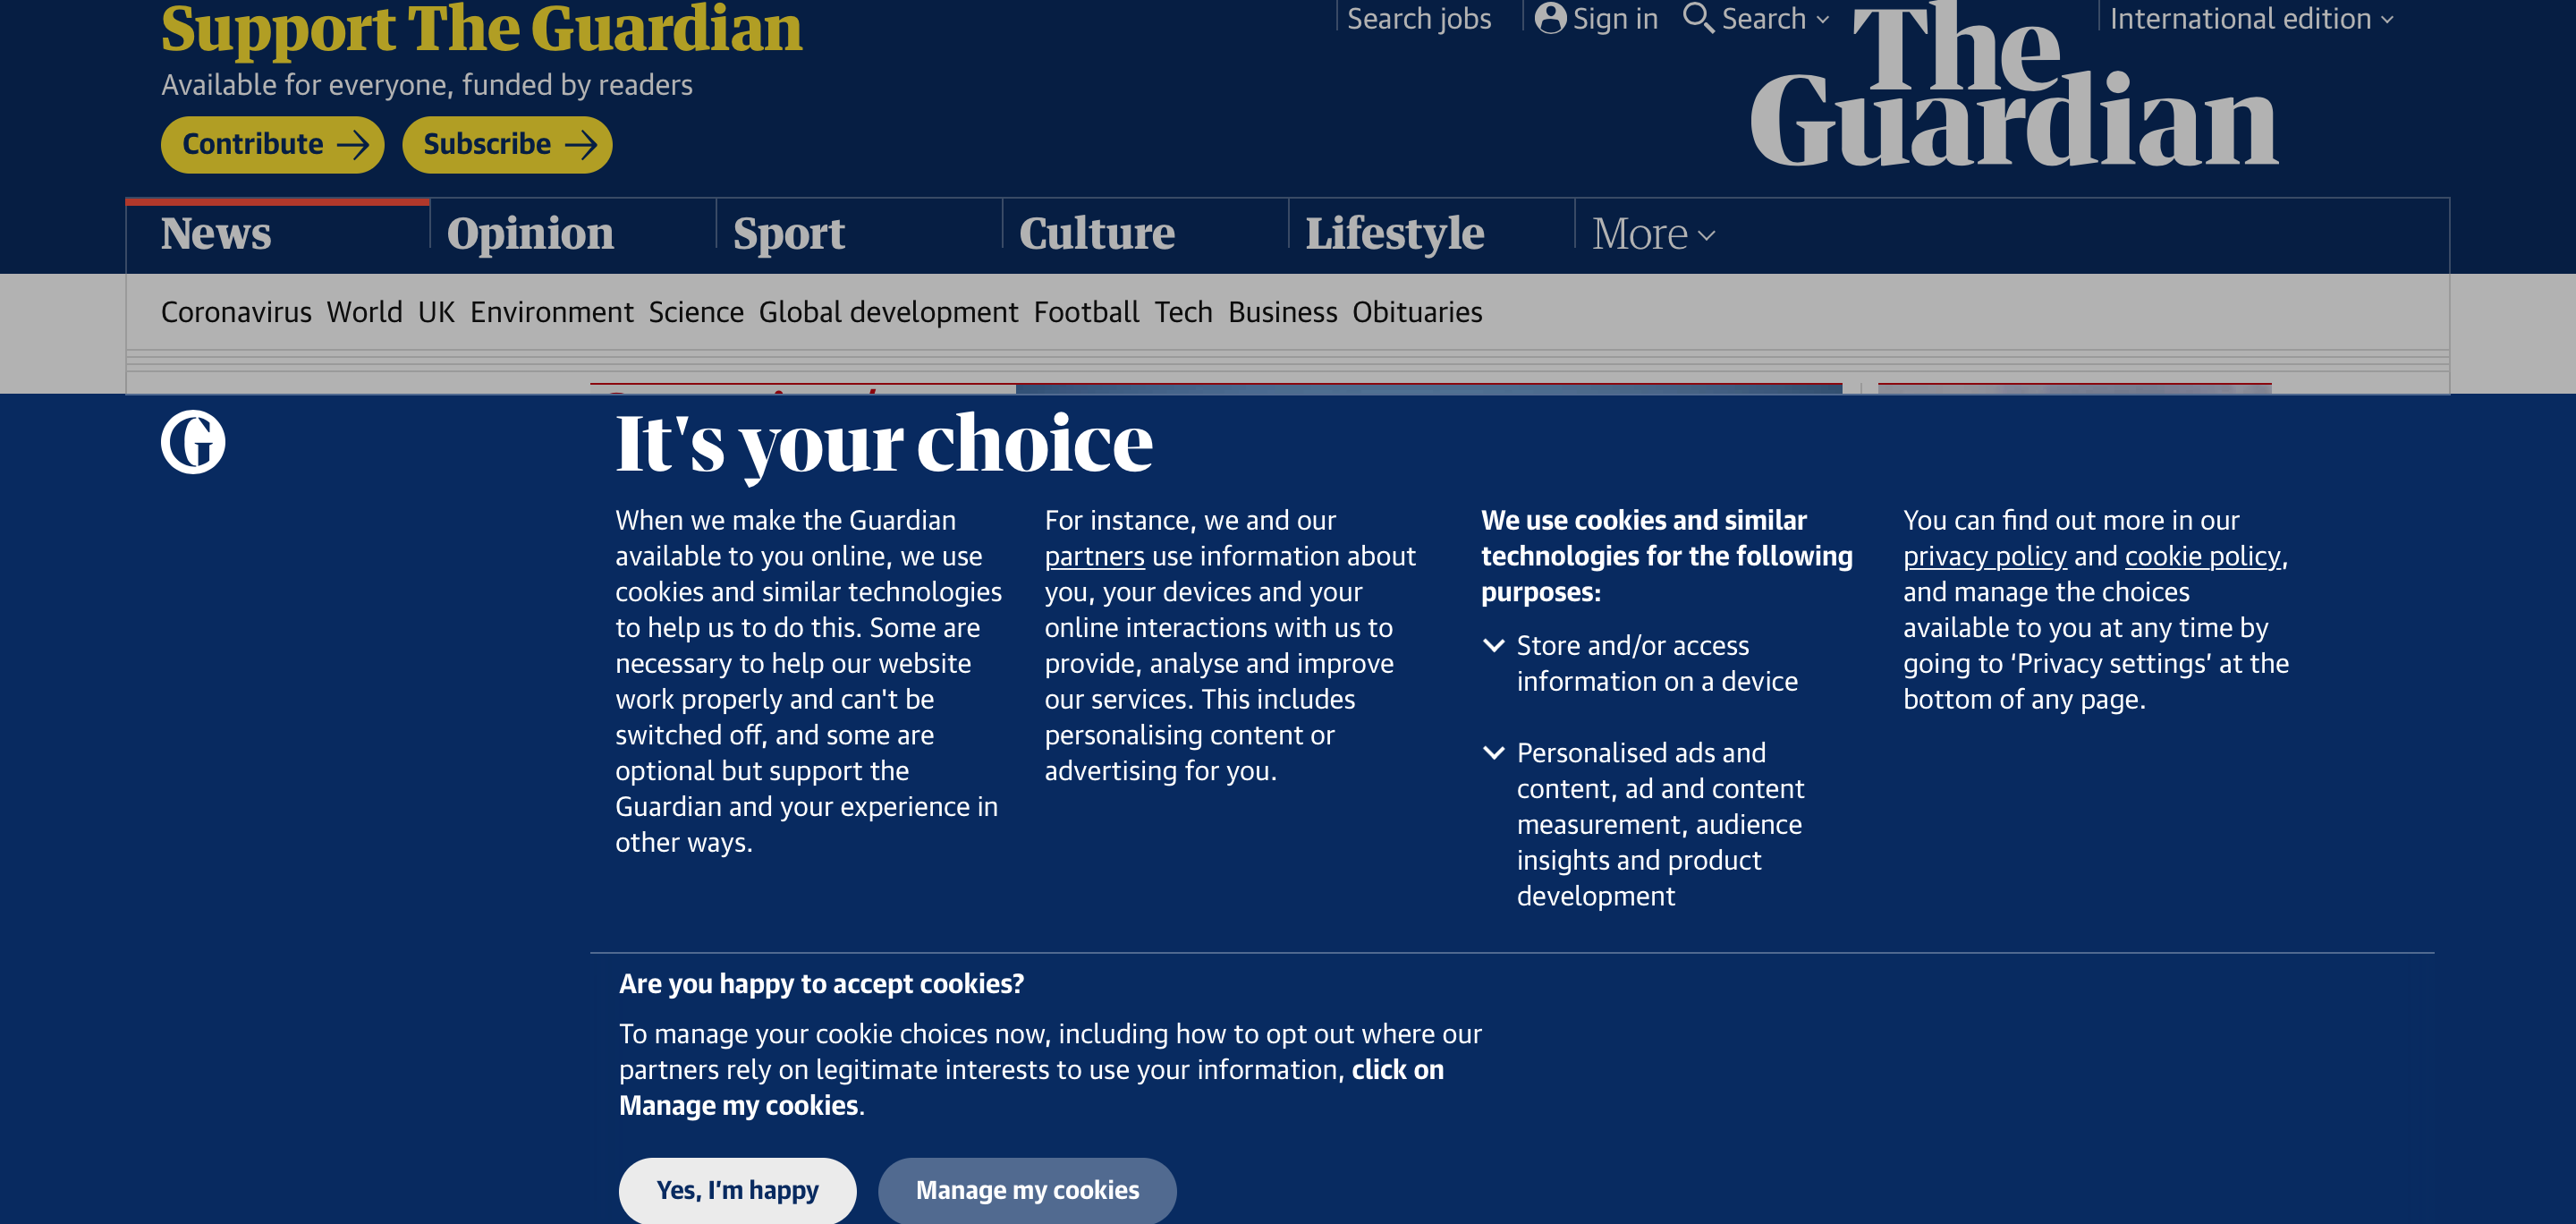
\includegraphics[width=\textwidth]{images/intro/york}
        \caption{The \say{bypass-able} cookie banner shown to York Uni's visitors.}
        \label{fig:intro_cookie_york}
    \end{subfigure}
    \caption{Two different cookie banner implementation approaches.}
    \label{fig:intro_cookie}
\end{figure}

As the GDPR states, when websites are storing tracking cookies on a user’s browser they are required to inform the visitor on how their data is going to be used and who is going to have access to them. Thus, websites implement cookie notices in order to inform users on their cookie policies and allow visitors to control their privacy settings via \say{privacy options} offered on the cookie banners e.g: \say{Accept all} or \say{Decline}.

Cookie notices can be a valuable tool for EU and UK and citizens to take control of their privacy online. However, they can also provide a powerful platform for websites to steer users towards privacy-intrusive choices in order to collect even more information on their visitors. 

\section{Motivation}
It is evident that the ubiquitous nature of cookie banners means that they are rapidly becoming part of a user’s daily web browsing experience. Especially after the GDPR came into force in 2018, more and more websites have added such notice. 

Since users increasingly have to deal with those privacy notices this project aims to provide a better understanding of cookie banners and the privacy options that they provide. More specifically, the research will focus on the types of cookie banners that users have to interact on a daily basis, whether visitors have a choice on whether they are being tracked and how the wording on those cookies notices may affect users’ perception of privacy and tracking.

\section{Aim}
This project focuses on the cookie banners in Greek as well as UK websites. These countries were chosen for 2 reasons. Firstly, they both adhere to very similar data protection laws, namely the GDPR and the Data Protection Act of 2018 and therefore, it is expected that most websites in these countries will have cookie notices. Secondly, both countries vastly differ in language and population size. Thus, potential differences in how the two populations experience the internet and the cookie banners are going to be highlighted.

The following list summarises the main goals of this project:

\begin{enumerate}
    \item \textbf{Users}: Develop a comprehensive understanding of the cookie banner landscape is useful not only for users but also for developing technologies that help users manage their privacy rights;
    \item \textbf{Governments}: Assist policymakers to have a better idea about the level of compliance to privacy laws by websites as well as the dark patterns that users encounter on a daily basis.
\end{enumerate}

\section{Research Questions}

In order to understand cookie banners better and how they affect the users’ internet experience, this project sets 7 research questions. These are summarised in the following list:

\begin{enumerate}[label=\textbf{RQ\arabic*}:, ref=RQ\arabic*, leftmargin=1.65cm]
    \item \label{rq:prevalence} What is the prevalence of cookie banners in popular websites across Greece and the UK? 
    \item \label{rq:options_avg} How many privacy options do cookie banners provide on average?
    \item \label{rq:direct_opt_out} How many cookie banners offer their users a direct \say{opt-out from tracking} option?
    \item \label{rq:no_options} How many cookie banners do not offer any option at all and inform their users that by \say{using this website, they agree to Third-Party Cookies and tracking}?
    \item \label{rq:common_ctas} What is the most common privacy option provided by the cookie banners? 
    \item \label{rq:manage_options_count} How many cookie banners allow their users to manage their privacy settings and control which vendors track them?
    \item \label{rq:common_privacy_txt} What is the average length of the cookie banner privacy text and what are the most common terms that are used to inform users about the use of cookie banners?
\end{enumerate}
    
\section{Contributions}

In order to answer the research questions set above, a number of novel methods and software was developed and a plethora of data was collected throughout the course of this project. All the contributions made are summarised in the following list:

\begin{enumerate}
    \item \label{contr_1} Developed an automated method of scraping and collecting cookie notices on a large scale, using OpenWPM;
    \item \label{contr_2} Conducted a more comprehensive study in Greece and the UK and collected a significantly larger dataset compared to other similar studies such as Habib et al.;
    \item \label{contr_3} Make the tools and data available so that similar research can be undertaken by other researchers in different countries.
\end{enumerate}

\end{document}